\documentclass[11pt]{charter}

% El títulos de la memoria, se usa en la carátula y se puede usar el cualquier lugar del documento con el comando \ttitle
\titulo{Sensor inteligente de vibración para mantenimiento predictivo} 

% Nombre del posgrado, se usa en la carátula y se puede usar el cualquier lugar del documento con el comando \degreename
\posgrado{Carrera de Especialización en Sistemas Embebidos} 
%\posgrado{Carrera de Especialización en Internet de las Cosas} 
%\posgrado{Carrera de Especialización en Intelegencia Artificial}
%\posgrado{Maestría en Sistemas Embebidos} 
%\posgrado{Maestría en Internet de las cosas}

% Tu nombre, se puede usar el cualquier lugar del documento con el comando \authorname
\autor{Ing. Martín Alejandro Mello Teggia} 

% El nombre del director y co-director, se puede usar el cualquier lugar del documento con el comando \supname y \cosupname y \pertesupname y \pertecosupname
\director{Esp. Lic. Pablo Castillo}
\pertenenciaDirector{CoNEA} 
% FIXME:NO IMPLEMENTADO EL CODIRECTOR ni su pertenencia
\codirector{} % si queda vacio no se deberíá incluir 
\pertenenciaCoDirector{}

% Nombre del cliente, quien va a aprobar los resultados del proyecto, se puede usar con el comando \clientename y \empclientename
\cliente{Dr. Ing. Cristian Muzzio}
\empresaCliente{HiTec S.R.L.}

% Nombre y pertenencia de los jurados, se pueden usar el cualquier lugar del documento con el comando \jurunoname, \jurdosname y \jurtresname y \perteunoname, \pertedosname y \pertetresname.
\juradoUno{Nombre y Apellido (1)}
\pertenenciaJurUno{pertenencia (1)} 
\juradoDos{Nombre y Apellido (2)}
\pertenenciaJurDos{pertenencia (2)}
\juradoTres{Nombre y Apellido (3)}
\pertenenciaJurTres{pertenencia (3)}
 
\fechaINICIO{23 de octubre de 2020}		%Fecha de inicio de la cursada de GdP \fechaInicioName
\fechaFINALPlanificacion{11 de diciembre de 2020} 	%Fecha de final de cursada de GdP
\fechaFINALTrabajo{22 de agosto de 2021}		%Fecha de defensa pública del trabajo final


\begin{document}

\maketitle
\thispagestyle{empty}
\pagebreak


\thispagestyle{empty}
{\setlength{\parskip}{0pt}
\tableofcontents{}
}
\pagebreak


\section{Registros de cambios}
\label{sec:registro}


\begin{table}[ht]
\label{tab:registro}
\centering
\begin{tabularx}{\linewidth}{@{}|c|X|c|@{}}
\hline
\rowcolor[HTML]{C0C0C0} 
Revisión & \multicolumn{1}{c|}{\cellcolor[HTML]{C0C0C0}Detalles de los cambios realizados} & Fecha      \\ \hline
0.1 & Creación del documento & 23/10/2020 \\ \hline
0.2 & Avances hasta punto 6 inclusive (sin user stories) & 06/11/2020 \\ \hline
0.3 & Agregado de user stories, y correcciones varias de secciones previas & 15/11/2020 \\ \hline
0.4      & Terminado hasta punto 12 inclusive, correcciones varias previas & 08/12/2020 \\ \hline
1.0      & Finalización del documento & 10/12/2020 \\ \hline
\end{tabularx}
\end{table}

\pagebreak



\section{Acta de constitución del proyecto}
\label{sec:acta}

\begin{flushright}
Buenos Aires, \fechaInicioName
\end{flushright}

\vspace{2cm}

Por medio de la presente se acuerda con el \authorname\hspace{1px} que su Trabajo Final de la \degreename\hspace{1px} se titulará ``\ttitle'', consistirá esencialmente en el prototipo preliminar de un sensor de vibración y temperatura, y tendrá un presupuesto preliminar estimado de 812 hs de trabajo y \textcolor{red}{\$XXX}, con fecha de inicio \fechaInicioName\hspace{1px} y fecha de presentación pública \fechaFinalName.

Se adjunta a esta acta la planificación inicial.

\vfill

% Esta parte se construye sola con la información que hayan cargado en el preámbulo del documento y no debe modificarla
\begin{table}[ht]
\centering
\begin{tabular}{ccc}
\begin{tabular}[c]{@{}c@{}}Ariel Lutenberg \\ Director posgrado FIUBA\end{tabular} & \hspace{2cm} & \begin{tabular}[c]{@{}c@{}}\clientename \\ \empclientename \end{tabular} \vspace{2.5cm} \\ 
\multicolumn{3}{c}{\begin{tabular}[c]{@{}c@{}} \supname \\ Director del Trabajo Final\end{tabular}} \vspace{2.5cm} \\
%\begin{tabular}[c]{@{}c@{}}\jurunoname \\ Jurado del Trabajo Final\end{tabular}     &  & \begin{tabular}[c]{@{}c@{}}\jurdosname\\ Jurado del Trabajo Final\end{tabular}  \vspace{2.5cm}  \\
%\multicolumn{3}{c}{\begin{tabular}[c]{@{}c@{}} \jurtresname\\ Jurado del Trabajo Final\end{tabular}} \vspace{.5cm}                                                                     
\end{tabular}
\end{table}



\newpage
\section{Descripción técnica-conceptual del proyecto a realizar}
\label{sec:descripcion}

\subsection*{Introducción general al tema}

El mantenimiento predictivo es indispensable en la industria farmacéutica, ya que la falla de un actuador puede implicar la pérdida de un lote completo de medicamentos, procesos que pueden consumir días enteros, y valiosos insumos.

Existe bibliografía que permite evaluar el desgaste de un motor mediante el análisis de sus vibraciones, procesando la información adquirida en el dominio de la frecuencia, y datos estadísticos en el dominio del tiempo.

En la empresa Hitec S.R.L. se desarrolló un sistema para realizar esta tarea, pero el objetivo del presente trabajo es trasladar el procesamiento al edge (MCU del sensor), y permitir la extracción de información de los sensores y no solo datos de mediciones.

Este producto se presenta como un sensor innovador, ya que las mediciones para mantenimiento predictivo se realizan mayormente offline. La incorporación de este sensor permite integrar el mantenimiento en la nube, lo que lo diferencia de la mayor parte de la competencia.

\subsection*{Descripción del producto a desarrollar}

El objetivo del hardware a desarrollar es adquirir y procesar datos de vibración y temperatura en el mismo sensor, para entregar información pre-procesada a una unidad central.

Para esto, el sensor deberá contar con un microcontrolador que realice las adquisiciones, procesamiento y comunicación de resultados, un circuito integrado que permita adquirir valores de vibración en tiempo real, un sensor de temperatura para medir las variaciones del dispositivo bajo análisis, y una memoria para almacenar datos de fabricación (y eventualmente calibración) independientes de la programación del microcontrolador. 

En la figura \ref{fig:diagramaBloques} se presenta un diagrama en bloques del sistema, donde puede verse las relaciones previamente mencionadas.

\begin{figure}[htpb]
\centering 
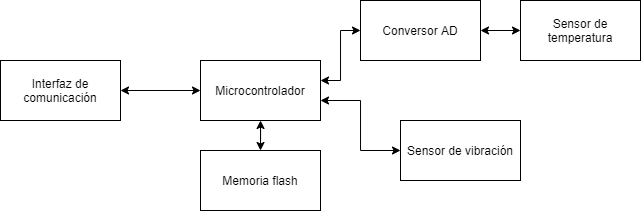
\includegraphics[width=1\textwidth]{./Figuras/diagramaBloques.png}
\caption{Diagrama en bloques del sistema}
\label{fig:diagramaBloques}
\end{figure}

El integrado de vibración debe ser encuestado a frecuencia constante, para garantizar el espaciamiento temporal de los valores medidos. El sensor de temperatura será encuestado solo para valores estadísticos, por lo que no será necesario un retardo estable entre mediciones.

El microcontrolador debe poder adquirir los valores, computar parámetros estadísticos, procesar el paso al dominio de la frecuencia, y extraer también información de esta representación. Es importante que el distanciamiento de muestras en el dominio del tiempo sea constante, para evitar el jitter en frecuencia. Finalmente, deberá almacenar los resultados obtenidos, e informarlos con una frecuencia configurable a un dispositivo central.

El sensor estará diseñado para soportar descargas electrostáticas, y otros eventos de compatibilidad electromagnética que puedan surgir en la industria. Para esto, se buscará cumplir con las siguientes normas:
\begin{itemize}
\item IEC 61000-4-2: ESD
\item IEC 61000-4-4: EFT
\item IEC 61000-4-5: Surge
\end{itemize}

De ser posible, también es de interés que el sensor sea ATEX, para poder operar en entornos que requieren que los dispositivos sean anti-explosivos.


\section{Identificación y análisis de los interesados}
\label{sec:interesados}

\begin{table}[ht]
\begin{tabularx}{\linewidth}{@{}|l|X|X|l|@{}}
\hline
\rowcolor[HTML]{C0C0C0} 
Rol           & Nombre y Apellido & Organización 	& Puesto 	\\ \hline
Auspiciante   &      Matías Montero             &       HiTec S.R.L.       	&      Contador  	\\ \hline
Cliente       & \clientename      &\empclientename	& Gerente I+D     	\\ \hline
Impulsor      & \clientename      &\empclientename	& Gerente I+D     	\\ \hline
Responsable   & \authorname       & FIUBA        	& Alumno 	\\ \hline
Colaboradores & Nicolás Dini & HiTec S.R.L. & Programador Senior \\ \newline 
			&	Luciano Gurevich  &    HiTec S.R.L.        	&  Data Scientist      	\\ \hline
Orientador    & \supname	      & \pertesupname 	& Director	Trabajo final \\ \hline
%Equipo        & - & - & -	\\ \hline
%Opositores    &           -        &       -       	&      -  	\\ \hline
Usuario final &       Martín Tomé            &  HiTec S.R.L.           	&  Jefe Servicio Técnico      	\\ \hline
\end{tabularx}
\end{table}


\begin{itemize}
\item Impulsor: \clientename tiene un conocimiento profundo de la industria, y las necesidades reales del producto.
\item Usuario Final: Martín Tomé tiene mucha experiencia con instalaciones, y puede ayudar a hacer más fácil de instalar y mantener el dispositivo, pero tiene poco tiempo disponible.
\item Colaborador: Nicolás Dini se ocupa de la interfaz de datos con la nube, el sensor tiene que poder finalmente comunicarse con su software.
\end{itemize}


\section{1. Propósito del proyecto}
\label{sec:proposito}

El propósito de este proyecto es desarrollar un sensor inteligente, capaz de adquirir y pre-procesar datos de un sensor de vibración, para poder utilizarlos para realizar mantenimiento predictivo sobre motores de la industria farmacéutica.

\section{2. Alcance del proyecto}
\label{sec:alcance}

%\begin{consigna}{red}
%¿Qué se incluye y que no se incluye en este proyecto?
%
%Se refiere al trabajo a hacer para entregar el producto o resultado especificado. 
%
%Explicitar todo lo quede comprendido dentro del alcance del proyecto.
%
%Explicitar además todo lo que no quede incluido (``El presente proyecto no incluye...'')
%
%\end{consigna}

El presente proyecto incluirá el desarrollo completo del hardware del sensor, e incluirá el desarrollo del firmware para la realización de las siguientes funciones:

\begin{itemize}
\item Adquisición de valores de aceleración en 3 ejes.
\item Procesamiento de parámetros estadísticos en el dominio del tiempo.
	\begin{itemize}
	\item Valores de aceleración RMS (sin continua).
	\item Valores de aceleración continua.
	\item Factor de cresta.
	\end{itemize}
\item Procesamiento de los valores en frecuencia.
\item Configuración del ancho de banda deseado en frecuencia.
\item Implementación de un código de tramas para comunicación con la unidad central.
\item Adquisición de valores de temperatura para análisis estadístico
\item Compatibilidad con el producto teBox (HiTec S.R.L.)
\end{itemize}

El firmware no incluirá la posibilidad de modificar la cantidad de muestras analizadas en frecuencia, ni la orientación de los ejes en función de la posición de instalación del sensor.

\section{3. Supuestos del proyecto}
\label{sec:supuestos}

Para el desarrollo del presente proyecto se supone que:

\begin{itemize}
\item La empresa HiTec se ocupará de la compra del material necesario para la fabricación del sensor, así como también de todos aquellos elementos requeridos para realizar las pruebas iniciales del producto.
\item Se dispondrá de las unidades necesarias del producto teBox para pruebas de compatibilidad, y que las unidades cumplen con sus especificaciones.
\item Se podrá consultar a Martín Tomé por cuestiones relacionadas a la instalación del sensor, a fin de desarrollar un dispositivo sencillo de utilizar desde su primera versión.
\item El laboratorio de pruebas de la empresa HiTec S.R.L. estará disponible durante toda la realización del proyecto, para realizar los ensayos necesarios con el instrumental presente.
\item El protocolo que se defina para comunicar al sensor será estandar, o contará con amplia documentación para su implementación en el microcontrolador.
\item Los componentes utilizados podrán ser adquiridos en Argentina, o traídos del exterior, durante la duración del proyecto.
\item Se podrán realizar las pruebas de compatibilidad electromagnética en el país durante la realización del proyecto.
\end{itemize}


\section{4. Requerimientos}
\label{sec:requerimientos}

\begin{enumerate}
\item Requerimientos de construcción del equipo
	\begin{enumerate}
	\item El gabinete deberá poder acoplarse a un motor sin necesidad de modificaciones.
	\item Se debe proveer con el mecanismo de acople una forma de medir la temperatura del motor.
	\item El gabinete será metálico (prioridad menor).
	\end{enumerate}
\item Requerimientos de conexionado
	\begin{enumerate}
	\item Línea de alimentación que contenga 5 V y permita extraer una corriente máxima de 200 mA.
	\item Línea de datos referido al mismo punto que la alimentación.
	\item El equipo debe contar con cables de alimentación y datos con polaridad.
	\item El equipo debe unificar los cables de alimentación y datos en un único cable
	 (prioridad menor).
	\end{enumerate}
\item Requerimientos asociados a la interfaz de comunicación
	\begin{enumerate}
	\item El sensor deberá poder comunicarse con el protocolo fijado por el producto teBox.
	\item El esquema de comunicación será maestro esclavo, con el sensor recibiendo ordenes y ejecutando acciones en base a ellas.
	\item El sensor deberá poder reprogramarse a través de la misma interfaz de datos (prioridad menor).
	\end{enumerate}
\item Requerimientos asociados a la medición
	\begin{enumerate}
	\item El sensor deberá poder adquirir valores de aceleración en 3 ejes ortogonales entre sí.
	\item El sensor deberá poder adquirir valores de temperatura del motor medido.
	\item Deberán poder extraerse datos estadísticos en el dominio del tiempo.
	\item Deberán poder extraerse datos en el dominio de la frecuencia.
	\item El sensor deberá guardar en una memoria flash externa información sobre máximos históricos, para evaluación durante servicios que se le ejecuten.
	\item Se deberá garantizar el espaciamiento temporal de los datos, para evitar jitter.
	\end{enumerate}
\item Requerimientos de validación
	\begin{enumerate}
	\item Cumplimiento norma IEC 61000-4-2: ESD.
	\item Cumplimiento norma IEC 61000-4-4: EFT.
	\item Cumplimiento norma IEC 61000-4-5: Surge.
	\end{enumerate}
\item Requerimientos de documentación
	\begin{enumerate}
	\item El código utilizará comentarios compatibles con Doxygen.
	\item Se proveerá un diagrama en bloques del procesamiento del microcontrolador.
	\item Se creará una entrada en la wiki de la empresa, con información de uso del firmware.
	\item Se generará un documento con el código de tramas para la comunicación de datos hacia y desde el microcontrolador.
	\end{enumerate}
\end{enumerate}


\section{Historias de usuarios (\textit{Product backlog})}
\label{sec:backlog}

\begin{itemize}
\item Como jefe de mantenimiento necesito conocer los valores de vibración de mi motor, para conocer el nivel de desgaste. (3 story points)
\item Como jefe de mantenimiento necesito conocer los valores de temperatura de mi motor, para detectar sobrecalentamientos. (1 story point)
\item Como unidad central de procesamiento necesito que el sensor se comunique con el protocolo propietario del producto teBox, para poder extraer datos. (3 story points)
\item Como algoritmo de mantenimiento predictivo necesito obtener valores estadísticos de vibración, para analizar la evolución de un motor en el tiempo. (5 story points)
\item Como algoritmo de mantenimiento predictivo necesito obtener los valores de vibración en el dominio de la frecuencia, para detectar desbalances y desalineamientos en sistemas mecánicos. (8 story points)
\item Como algoritmo de mantenimiento predictivo necesito conocer si el sensor fue movido luego de instalarse, para evitar realizar comparaciones de datos inconsistentes. (5 story points)
\end{itemize}


\section{5. Entregables principales del proyecto}
\label{sec:entregables}

Los entregables principales del proyecto serán:
\begin{itemize}
\item Manual de uso
\item Diagrama esquemático
\item Código fuente
\item Diagrama de instalación
\item Certificados de compatibilidad electromagnética
\item Informe final

\end{itemize}


\section{6. Desglose del trabajo en tareas}
\label{sec:wbs}

\begin{enumerate}
\item Gestión del proyecto (88 hs)
	\begin{enumerate}
	\item Análisis de bibliografía existente y opciones desplegadas en el mercado (40 hs)
	\item Elaboración de la planificación del proyecto (40 hs)
	\item Definición de los casos de prueba (8 hs)
	\end{enumerate}
\item Diseño de hardware (104 hs)
	\begin{enumerate}
	\item Diseño de la arquitectura de hardware a utilizar (24 hs)
	\item Análisis y elección de un gabinete (16 hs)
	\item Diseño del PCB (40 hs)
	\item Elección de conectores (16 hs)
	\item Revisión del CAD del gabinete con el del PCB y los conectores (8 hs)
	\end{enumerate}
\item Desarrollo de firmware (232 hs)
	\begin{enumerate}
	\item Desarrollo de biblioteca para manejo de periféricos necesarios (16 hs)
	\item Desarrollo de biblioteca para adquisición y almacenamiento de valores de los sensores (40 hs)
	\item Procesamiento de valores para obtención de estadísticos (16 hs)
	\item Implementación de algoritmo de FFT (16 hs)
	\item Procesamiento de valores en el dominio de la frecuencia (40 hs)
	\item Programación de interfaz para comunicación con teBox (40 hs)
	\item Procesamiento de valores históricos, e interacción con memoria flash externa (32 hs)
	\item Ajuste de valores contra un patrón (32 hs)
	\end{enumerate}
\item Producción de prototipo (56 hs)
	\begin{enumerate}
	\item Logística de fabricación de prototipo de PCB (8 hs)
	\item Adquisición de componentes de conexionado (16 hs)
	\item Logística de recepción de elementos (8 hs)
	\item Ensamblado de prototipos (16 hs)
	\item Medición de tensiones y conexionado en prototipo ensamblado (8 hs)
	\end{enumerate}
\item Testing y depuración (120 hs)
	\begin{enumerate}
	\item Generación de muestras para casos de prueba (40 hs)
	\item Validación de los valores obtenidos contra muestras patrón (24 hs)
	\item Ensayos de compatibilidad electromagnética (16 hs)
	\item Modificaciones en base a errores detectados (40 hs)
	\end{enumerate}
\item Documentación (112 hs)
	\begin{enumerate}
	\item Elaboración de manuales (56 hs)
	\item Documentación en wiki de la empresa (32 hs)
	\item Elaboración de diagrama de flujo del programa (24 hs)
	\end{enumerate}
\item Cierre de proyecto (100 hs)
	\begin{enumerate}
	\item Gestión del proceso de cierre del proyecto (8 hs)
	\item Elaboración de informe final (64 hs)
	\item Elaboración de la presentación (24 hs)
	\item Presentación del informe final (4 hs)
	\end{enumerate}
\end{enumerate}

Cantidad total de horas: 812 hs


\section{7. Diagrama de Activity On Node}
\label{sec:AoN}

\begin{figure}[htpb]
\centering 
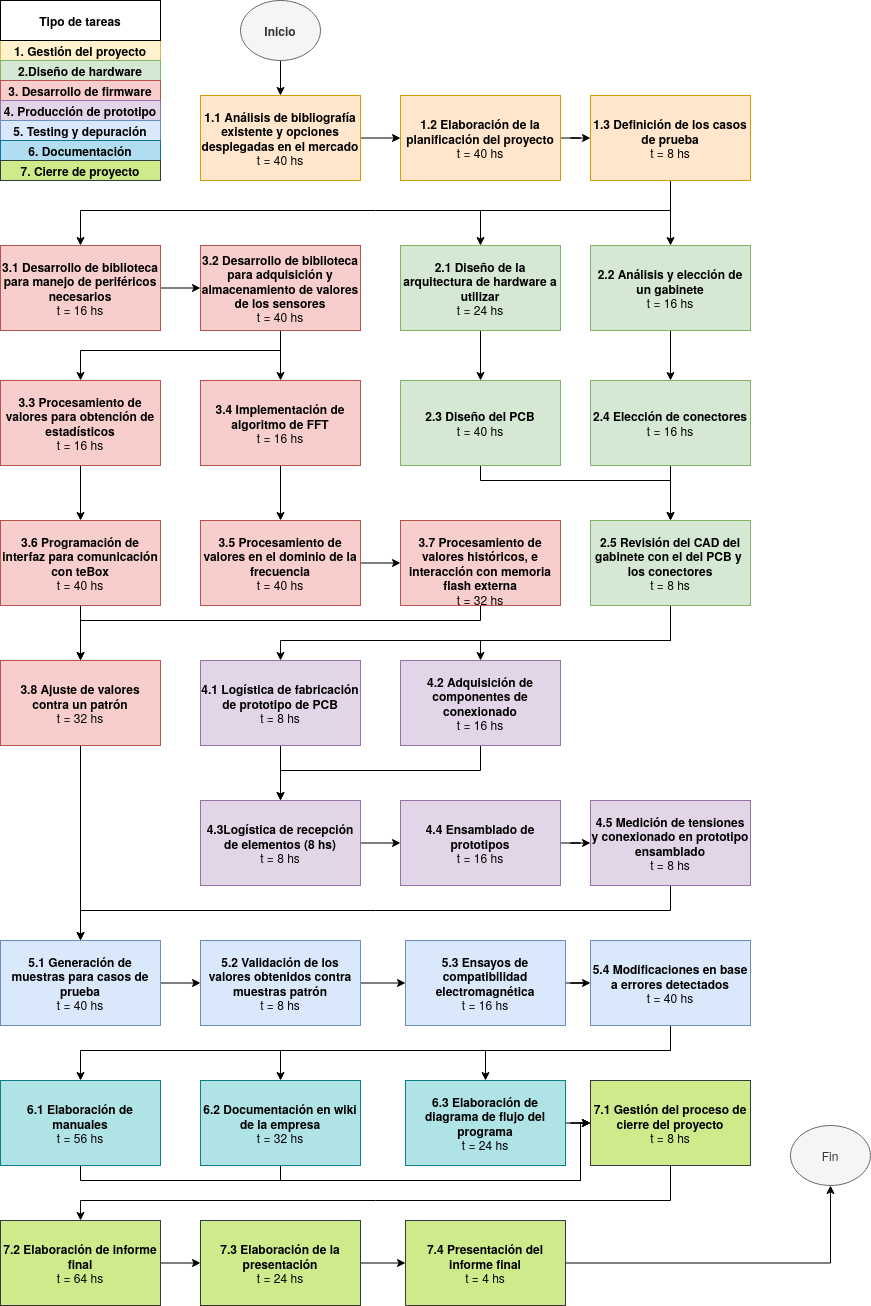
\includegraphics[width=.8\textwidth]{./Figuras/ActivityOnNode.png}
\caption{Diagrama de Activity on Node}
\label{fig:AoN}
\end{figure}


\section{8. Diagrama de Gantt}
\label{sec:gantt}

Debido al tamaño del proyecto, se exportó el diagrama de gantt indicando solo los números de tareas del WBS, y por separado se provee un listado del WBS para poder corroborar la correspondencia con el diagrama de AoN y WBS previo.

\begin{figure}[htpb]
\centering 
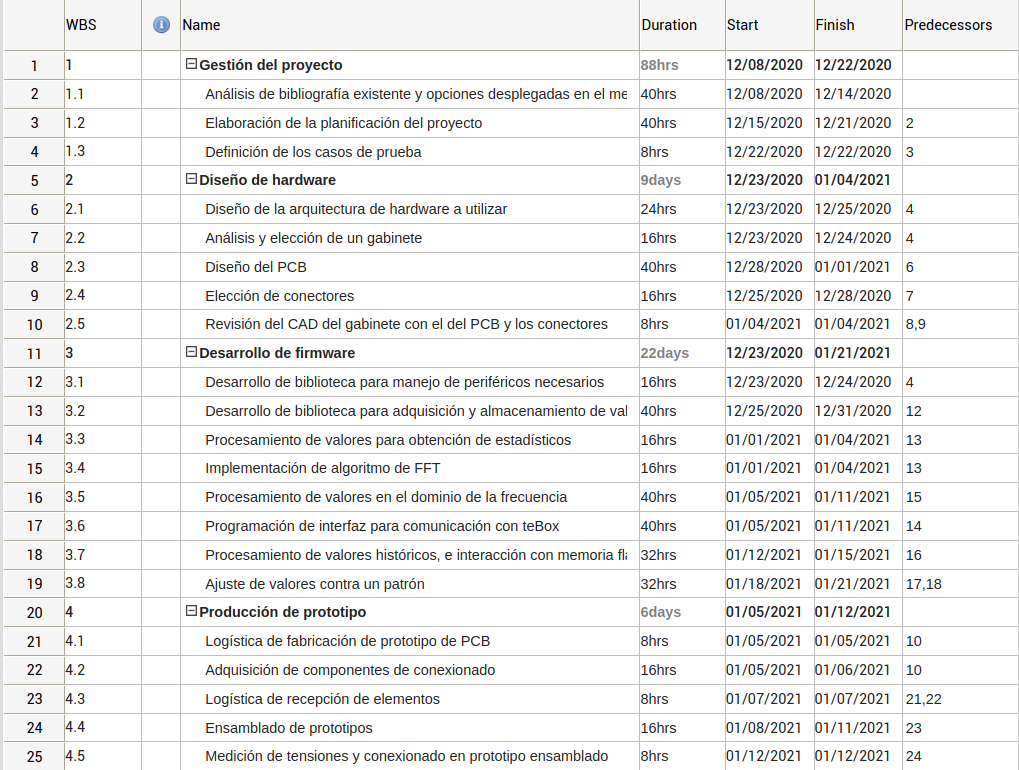
\includegraphics[width=.8\textwidth]{./Figuras/wbs1.png}
%\caption{WBS - parte 1}
\label{fig:wbs1}
\end{figure}

\begin{figure}[htpb]
\centering 
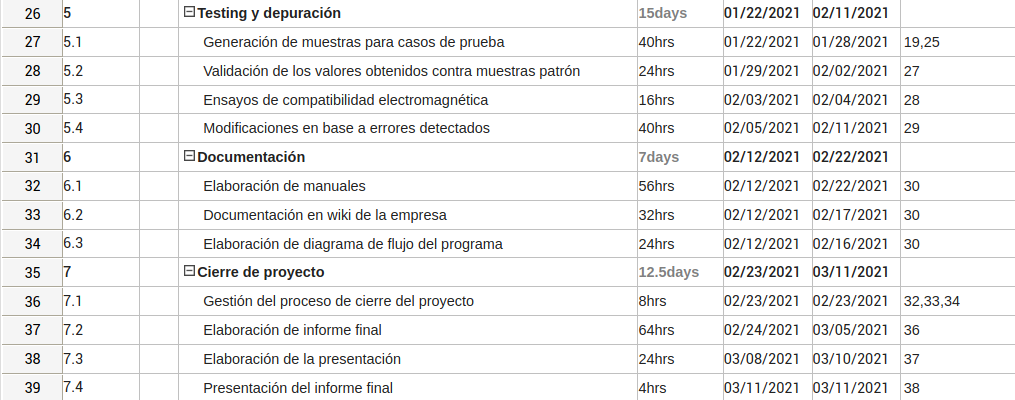
\includegraphics[width=.8\textwidth]{./Figuras/wbs2.png}
\caption{WBS}
\label{fig:wbs2}
\end{figure}

\begin{figure}[htpb]
\centering 
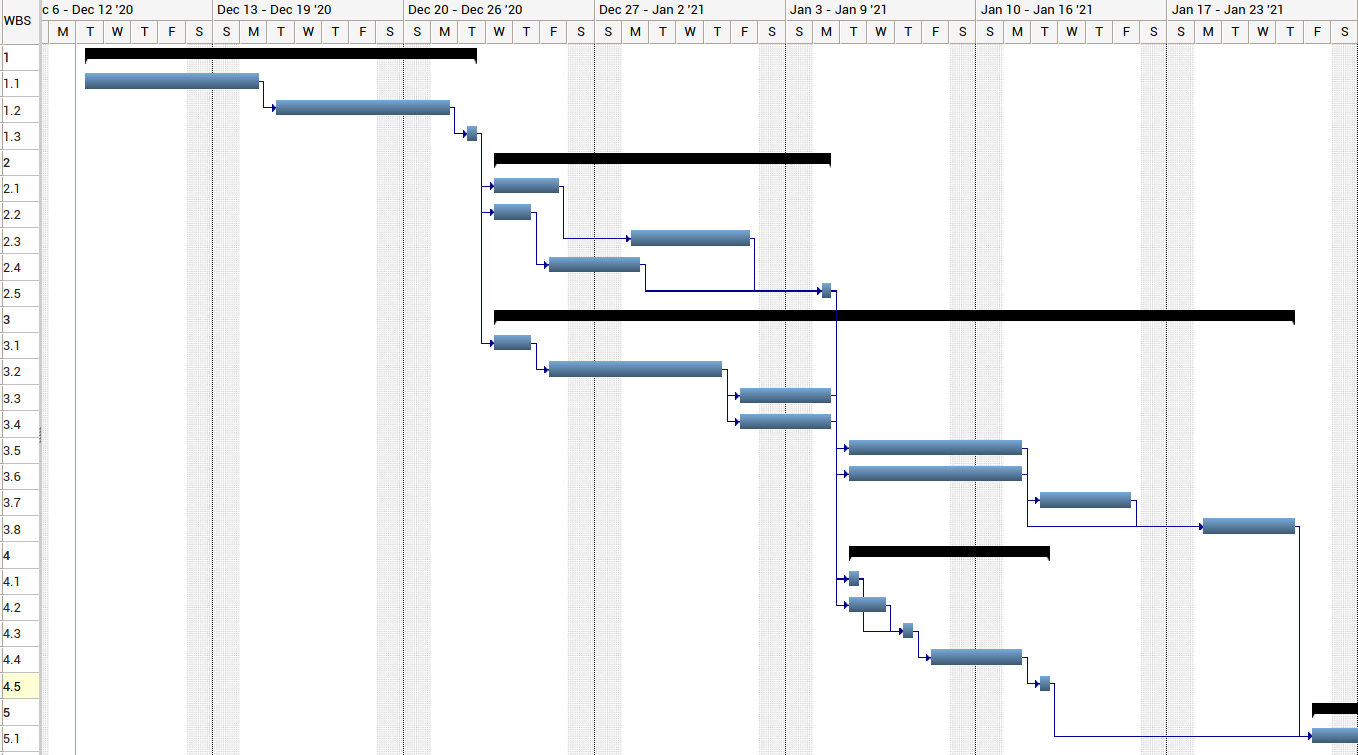
\includegraphics[width=1\textwidth]{./Figuras/gantt1.png}
\caption{Diagrama de Gantt - parte 1}
\label{fig:gantt1}
\end{figure}

\begin{figure}[htb]
\centering 
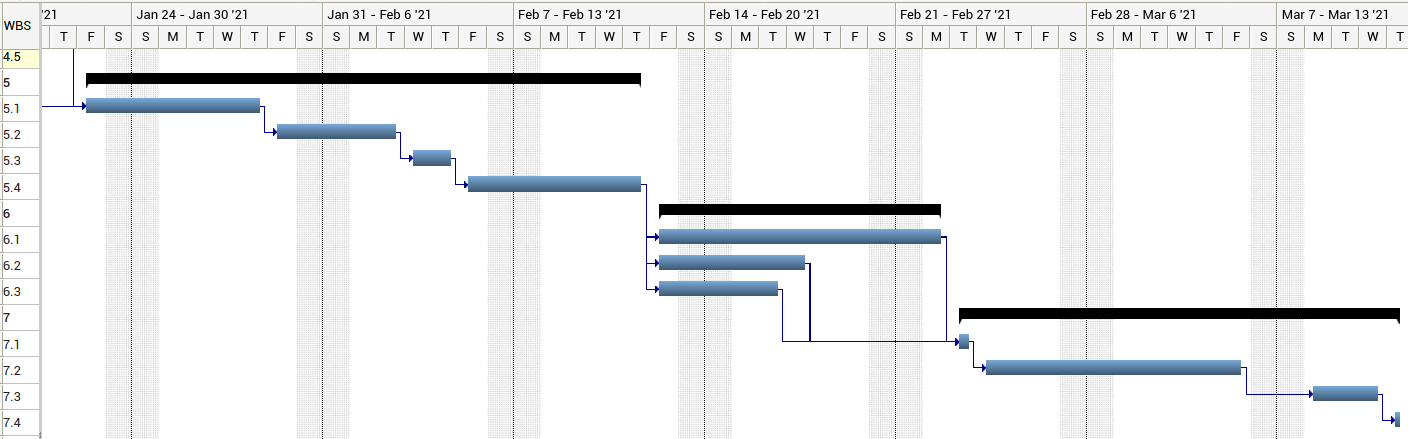
\includegraphics[width=1\textwidth]{./Figuras/gantt2.png}
\caption{Diagrama de Gantt - parte 2}
\label{fig:gantt2}
\end{figure}


\section{9. Matriz de uso de recursos de materiales}
\label{sec:recursos}


%\begin{table}
%\label{tab:recursos}
%\centering
%\begin{tabularx}{\linewidth}{@{}|c|X|X|X|X|c|@{}}
%\hline
%\cellcolor[HTML]{C0C0C0} & \cellcolor[HTML]{C0C0C0} & \multicolumn{4}{c|}{\cellcolor[HTML]%{C0C0C0}Recursos requeridos (horas)} \\ \cline{3-6} 
%\multirow{-2}{*}{\cellcolor[HTML]{C0C0C0}\begin{tabular}[c]{@{}c@{}}Código\\ WBS\end{tabular}} & \multirow{-2}{*}{\cellcolor[HTML]{C0C0C0}\begin{tabular}[c]{@{}c@{}}Nombre \\ tarea%\end{tabular}} & PC & TeBox & TeSensor-VT & Laboratorio de mediciones \\ \hline
%1 & Gestión del proyecto & 88 &  &  &  \\ \hline
%2 & Diseño de hardware & 104 &  &  &  \\ \hline
%3 & Desarrollo de firmware & 232 & 40 &  &  \\ \hline
%4 & Producción de prototipo & 56 &  &  & 24 \\ \hline
%5 & Testing y depuración & 120 & 80 & 80 & 64 \\ \hline
%6 & Documentación & 112 &  &  &  \\ \hline
%7 & Cierre de proyecto & 100 & 28 & 28 & 24 \\ \hline
%\end{tabularx}%
%\end{table}

\begin{figure}[htpb]
\centering 
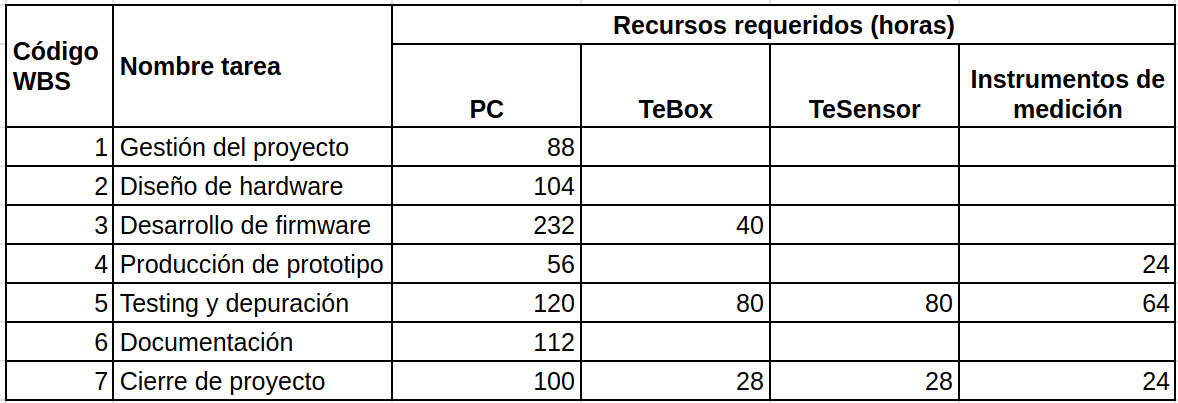
\includegraphics[width=1\textwidth]{./Figuras/matrizUsoRecursos.png}
\caption{Matriz de uso de recursos}
\label{fig:matrizRecursos}
\end{figure}


\section{10. Presupuesto detallado del proyecto}
\label{sec:presupuesto}

\begin{figure}[htpb]
\centering 
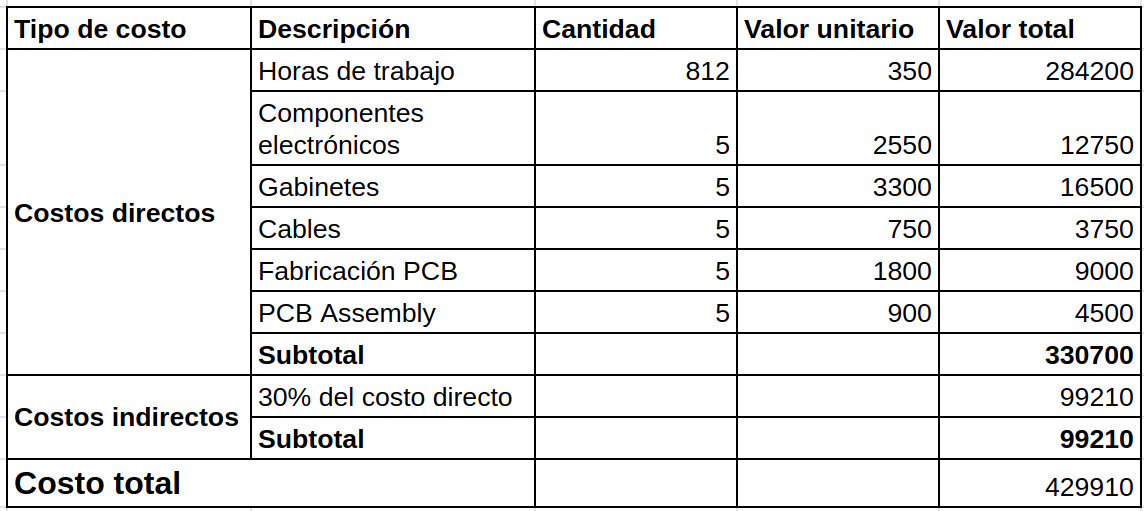
\includegraphics[width=1\textwidth]{./Figuras/costos.png}
\caption{Presupuesto detallado del proyecto}
\label{fig:costos}
\end{figure}


\section{11. Matriz de asignación de responsabilidades}
\label{sec:responsabilidades}

\begin{figure}[h]
\centering 
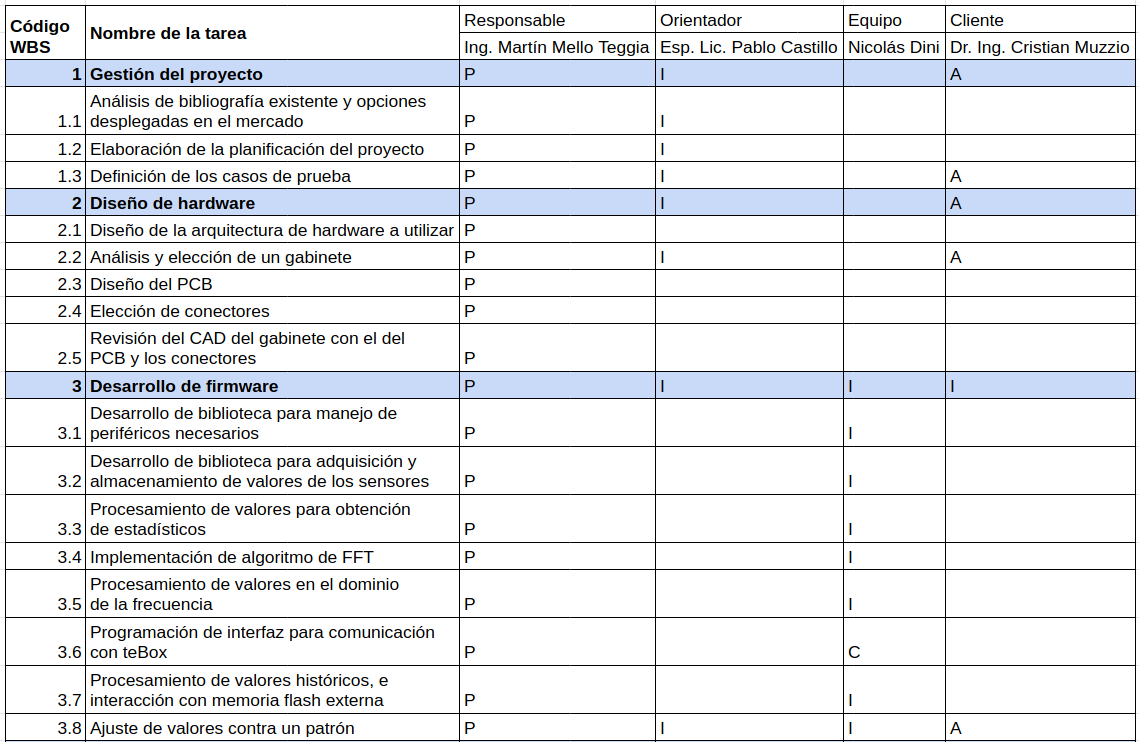
\includegraphics[width=1\textwidth]{./Figuras/responsabilidades1.png}
\caption{Matrìz de asignación de responsabilidades - parte 1}
\label{fig:responsabilidades1}
\end{figure}

\begin{figure}[h]
\centering 
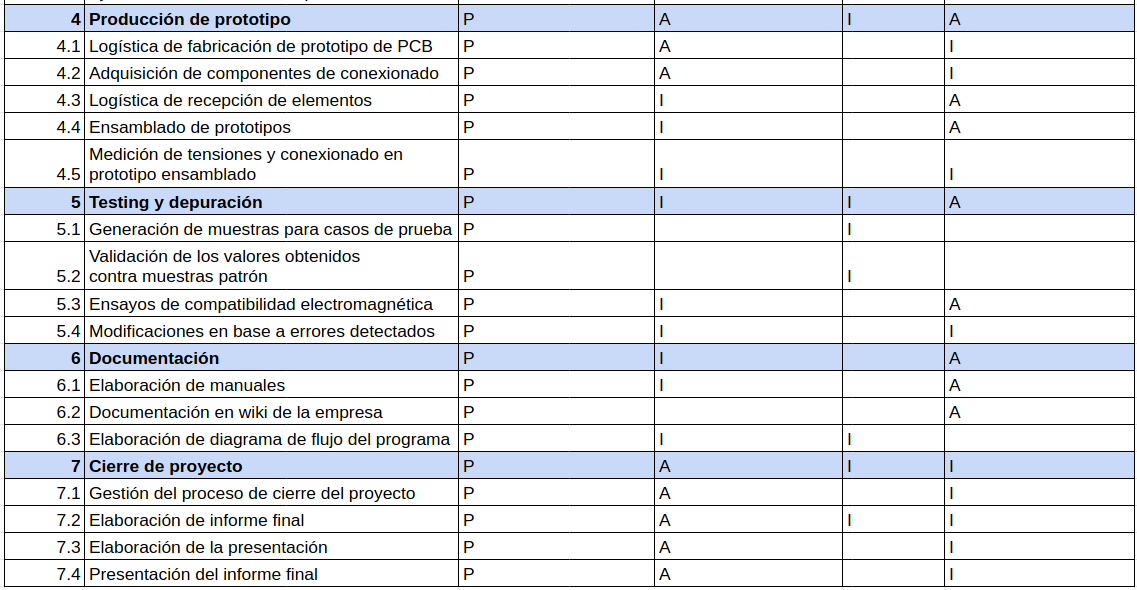
\includegraphics[width=1\textwidth]{./Figuras/responsabilidades2.png}
\caption{Matrìz de asignación de responsabilidades - parte 2}
\label{fig:responsabilidades2}
\end{figure}

Referencias:
\begin{itemize}
\item P = Responsabilidad Primaria
\item S = Responsabilidad Secundaria
\item A = Aprobación
\item I = Informado
\item C = Consultado
\end{itemize}

\section{12. Gestión de riesgos}
\label{sec:riesgos}

a) Identificación de los riesgos y estimación de sus consecuencias:

Riesgo 1: El cliente informa que los requerimientos no están cumplidos en el producto.
\begin{itemize}
\item Severidad (S): 9. Si no se cumplen las espectativas del cliente, se dificulta la comercialización del producto.
\item Ocurrencia (O): 4. La relación con el cliente hace que el mismo  vaya a involucrarse durante el desarrollo del producto, lo que implica una probabilidad media a baja de ocurrencia.
\end{itemize}

Riesgo 2: Detectar errores en el PCB fabricado.
\begin{itemize}
\item Severidad (S): 7. Los errores detectados pueden ser salvables o no, pero reducen la robustez del producto. La severidad es media-alta, ya que pueden existir errores en todas los ordenes de severidad.
\item Ocurrencia (O): 7. En todo desarrollo donde quien revisa los desarrollos es el mismo que los lleva adelante, es muy probable que existan errores de diseño.
\end{itemize}

Riesgo 3: Pérdida del software desarrollado.
\begin{itemize}
\item Severidad (S): 7. La perdida de código puede genera retrasos importantes en el desarrollo del producto.
\item Ocurrencia (O): 1. El uso de repositorios hace que este riesgo se vea notablemente reducido, llevandolo a un punto de ocurrencia muy bajo.
\end{itemize}

Riesgo 4: Falla de la planificación en la estimación de tiempos.
\begin{itemize}
\item Severidad (S): 8. Una falla en la estimación de tiempos genera retrasos en el proyecto completo, y es un riesgo severo.
\item Ocurrencia (O): 3. La planificación extensa de las tareas a realizar, y la realización previa de proyectos similares llevan a una baja probabilidad de ocurrencia.
\end{itemize}

Riesgo 5: Problemas en la importación de los componentes
\begin{itemize}
\item Severidad (S): 10. Si no se pueden importar los componentes, no se puede fabricar el producto.
\item Ocurrencia (O): 6. Durante el año 2020 cambiaron numerosas veces las reglamentaciones, y elementos que podían ser ingresados previamente al país dejaron de poder pedirse por courier.
\end{itemize}


b) Tabla de gestión de riesgos:

\begin{table}[htpb]
\centering
\begin{tabularx}{\linewidth}{@{}|X|c|c|c|c|c|c|@{}}
\hline
\rowcolor[HTML]{C0C0C0} 
Riesgo & S & O & RPN & S* & O* & RPN* \\ \hline
1- Requerimientos incumplidos   &  9 & 4  &  36   &  9  &  1  &  9    \\ \hline
2- Errores en el PCB   &  7 & 7  &  49   &  4  &  4  &   16   \\ \hline
3- Perdida de software       &  7 & 1  &  7   & 7   &  1  &  7    \\ \hline
4- Falla de tiempos      & 8  &  3 &  24   & 8   & 3   &  24    \\ \hline
5- Problemas de importación  & 10  & 5  &  50   &  10  &  2  &  20    \\ \hline
\end{tabularx}%
\end{table}

Criterio adoptado: 
Se tomarán medidas de mitigación en los riesgos cuyos números de RPN sean mayores a 30

Nota: los valores marcados con (*) en la tabla corresponden luego de haber aplicado la mitigación.

c) Plan de mitigación de los riesgos que originalmente excedían el RPN máximo establecido:
 
Riesgo 1: El cliente informa que los requerimientos no están cumplidos en el producto.
\begin{itemize}
\item Plan de mitigación: Se firmarán con el cliente especificaciones claras a ser cumplidas, y los procesos de validación de las mismas.
\item Severidad (S): 9. Sigue siendo igual de serio el riesgo de que no se cumpla una especificación.
\item Probabilidad de ocurrencia (O): 1. Al dejar documentos firmados con la forma de evaluación, se elimina cualquier subjetividad que pueda existir sobre el cumplimiento del producto.
\end{itemize}
 
Riesgo 2: Detectar errores en el PCB fabricado.
\begin{itemize}
\item Plan de mitigación: Se reserva tiempo para realizar pruebas, y realizar un rediseño en base a los errores detectados.
\item Severidad (S): 4. Los errores más serios no podrán pasar sin ser detectados de las pruebas, por lo que los errores remanentes serán de menor severidad.
\item Probabilidad de ocurrencia (O): 4. Al contar con una instancia más de iteración, se reduce mucho la cantidad de errores que podrán resultar en el producto final.
\end{itemize}
 
Riesgo 5: Problemas de importación.
\begin{itemize}
\item Plan de mitigación: Se están desarrollando fabricantes locales de PCB, y contacto con importadores de componentes.
\item Severidad (S): 10. La severidad de no conseguir los elementos necesarios sigue siendo máxima, ya que imposibilita el desarrollo del producto.
\item Probabilidad de ocurrencia (O): 2. El agregado de nuevos canales para la obtención de los materiales necesarios vuelve poco probable que no se los pueda adquirir.
\end{itemize}

\section{13. Gestión de la calidad}
\label{sec:calidad}

\begin{itemize}
\item Grupo de requerimientos 1: Gestión del proyecto.
\begin{itemize}
\item Verificación: Se revisará la planificación, para confirmar que los tiempos estimados fueron cumplidos.
\item Validación: La fecha de entrega permitirá validar la planificación.
\end{itemize}
\end{itemize}

\begin{itemize}
\item Grupo de requerimientos 2: Diseño de hardware.
\begin{itemize}
\item Verificación: Se verificará el CAD del gabinete con el del PCB y los conectores para confirmar la comptabilidad del hardware diseñado.
\item Validación: Se enviarán los documentos CAD al cliente, para que valide el diseño completo.
\end{itemize}
\end{itemize}


\begin{itemize}
\item Grupo de requerimientos 3: Desarrollo de firmware.
\begin{itemize}
\item Verificación: Se verificará que desde la teBox puedan obtenerse datos del sensor de vibración, y que los mismos se correspondan con el eje de la gravedad al modificar la orientación del gabinete.
\item Validación: Se subirán a una plataforma web valores medidos por el sensor, y se le proporcionará al cliente acceso a los mismos.
\end{itemize}
\end{itemize}


\begin{itemize}
\item Grupo de requerimientos 4: Producción de prototipo.
\begin{itemize}
\item Verificación: Se comprobará que el prototipo ensamblado cumpla con los requerimientos establecidos.
\item Validación: Se enviará un video en funcionamiento del prototipo al cliente, en el cual se mostrará el prototipo funcionando.
\end{itemize}
\end{itemize}


\begin{itemize}
\item Grupo de requerimientos 5: Testing y depuración.
\begin{itemize}
\item Verificación: Se ensayará el prototipo en el INTI, para verificar los requerimientos de EMC establecidos. También se evaluaran los casos de prueba previamente establecidos.
\item Validación: Se enviarán los certificados de las pruebas de EMC, junto con los resultados de los casos de prueba al cliente.
\end{itemize}
\end{itemize}


\begin{itemize}
\item Grupo de requerimientos 6 : Documentación.
\begin{itemize}
\item Verificación: Se revisará haber cumplido con todos los requisitos de documentación establecidos en el proyecto.
\item Validación: Se enviarán al cliente los documentos finales redactados.
\end{itemize}
\end{itemize}


\section{14. Comunicación del proyecto}
\label{sec:comunicaciones}

El responsable de todas las comunicaciones será el responsable del proyecto. El plan de comunicación del proyecto es el siguiente:

\begin{table}[htpb]
\centering
\begin{tabularx}{\linewidth}{@{}|X|C{2.4cm}|C{3cm}|C{1.8cm}|C{2cm}|C{2.1cm}|@{}}
\hline
\rowcolor[HTML]{C0C0C0} 
\multicolumn{6}{|c|}{\cellcolor[HTML]{C0C0C0}PLAN DE COMUNICACIÓN DEL PROYECTO}           \\ \hline
\rowcolor[HTML]{C0C0C0} 
¿Qué comunicar? & Audiencia & Propósito & Frecuencia & Método de comunicac. & Responsable \\ \hline 
Definición de la planificación del proyecto & Todos los interesados & Confirmar el alcance del proyecto & Una vez (al inicio del proyecto) & Correo electrónico y llamada telefónica & Martín Mello Teggia \\ \hline
Avance del proyecto & Orientador y cliente & Informar el estado y recibir sugerencias & Semanal & Correo electrónico & Martín Mello Teggia \\ \hline
Resolución de conflictos & Orientador y cliente & Plantear problemas y recoger posibles soluciones & Cada vez que sea necesario & Video conferencia & Martín Mello Teggia \\ \hline
Consultas & Colaborador & Información del producto teBox & Cada vez que sea necesario & Sistemea de chat de la empresa & Martín Mello Teggia \\ \hline
Prototipo ensamblado & Todos los interesados & Validación del diseño & Una vez & Correo electrónico & Martín Mello Teggia \\ \hline
Finalización del proyecto & Todos los interesados & Validación del producto & Una vez (al finalizar el proyecto) & Correo electrónico y video conferencia & Martín Mello Teggia \\ \hline
\end{tabularx}
\end{table}

\section{15. Gestión de compras}
\label{sec:compras}

En este caso, todas las compras se realizarán a través del departamento de compras de la empresa HiTec S.R.L..

Todas estas compras se llevarán a cabo de acuerdo a los criterios utilizados por la empresa, y no forman parte del presente trabajo.

\section{16. Seguimiento y control}
\label{sec:seguimiento}


\begin{longtable}{|m{1cm}|m{3.5cm}|m{2.2cm}|m{2cm}|m{3cm}|m{1.5cm}|}
\hline
\rowcolor[HTML]{C0C0C0} 
\multicolumn{6}{|c|}{\cellcolor[HTML]{C0C0C0}SEGUIMIENTO DE AVANCE}                                                                       \\ \hline
\rowcolor[HTML]{C0C0C0} 
Tarea del WBS 			& Indicador de avance & Frecuencia de reporte & Resp. de seguimiento & Persona a ser informada & Método de comunic. \\ \hline
\endfirsthead

\hline
\rowcolor[HTML]{C0C0C0} 
\multicolumn{6}{c}{\cellcolor[HTML]{C0C0C0}SEGUIMIENTO DE AVANCE}                                                                       \\ \hline
\rowcolor[HTML]{C0C0C0} 
Tarea del WBS 			& Indicador de avance & Frecuencia de reporte & Resp. de seguimiento & Persona a ser informada & Método de comunic. \\ \hline
\endhead

\multicolumn{6}{c}{Continúa}
\endfoot

\endlastfoot
1.x & \# tareas terminadas & Única vez (al comienzo) & \authorname & \clientename, \supname & Correo electrónico y llamada telefónica \\ \hline
2.x & \% del hardware terminado & Semanalmente & \authorname & \clientename, \supname & Correo electrónico \\ \hline
3.x & \% de las funciones implementadas & Semanalmente & \authorname & \clientename, \supname & Correo electrónico \\ \hline
4.x & \% componentes obtenidos & Semanalmente & \authorname & \clientename, \supname & Correo electrónico \\ \hline
5.1 & \% casos de prueba evaluados & Semanalmente & \authorname & \clientename, \supname & Correo electrónico \\ \hline
5.2 & \% muestras evaluadas & Única vez & \authorname & \clientename, \supname & Correo electrónico \\ \hline
5.3 & \% pruebas superadas & Única vez & \authorname & \clientename, \supname & Correo electrónico \\ \hline
6.x & \% archivos de documentación entregados & Semanalmente & \authorname & \clientename, \supname & Correo electrónico \\ \hline

\end{longtable}


\section{17. Procesos de cierre}    
\label{sec:cierre}

Tomando la planificación inicial como punto de partida, se evaluará cual fue el grado de cumplimiento de cada tarea. Para aquellas que no pudieron ser cumplidas, o que tomaron al menos un 20\% adicional de tiempo, se realizará una descripción de los problemas encontrados para referencia futura.

\begin{itemize}
\item Se entregará al cliente toda la documentación del proyecto, de acuerdo a lo pactado en la planificación, para ser utilizado como el cliente crea conveniente.
\item Se realizará una presentación en la que se expondrá el trabajo realizado, para ser presentado frente a las autoridades de la carrera de especialización.
\item Se agradecerá a todos los que colaboraron en la realización del proyecto, principalmente a los colaboradores.
\end{itemize}

\end{document}
